%This is the homework 1 latex file.

\documentclass{article}
\usepackage{amsfonts}
\usepackage{amssymb}
\usepackage{graphicx}
\usepackage{mathtools}
\usepackage{color}
\usepackage[margin=2cm]{geometry}
\DeclarePairedDelimiter\ceil{\lceil}{\rceil}
\DeclarePairedDelimiter\floor{\lfloor}{\rfloor}


%add my usual shit to the preamble here.




\begin{document}

\begin{enumerate}
    %1
    \item
    \begin{enumerate}
        %1a
        \item $D, M, B, K, V, S, H, Q, F, C, L, A, U, R$\\
            Solution path: $D{\rightarrow}M{\rightarrow}B{\rightarrow}K{\rightarrow}V{\rightarrow}S{\rightarrow}H{\rightarrow}Q{\rightarrow}F{\rightarrow}C{\rightarrow}L{\rightarrow}U{\rightarrow}R$

        %1b
        \item \textcolor{white}{.}\\ 
            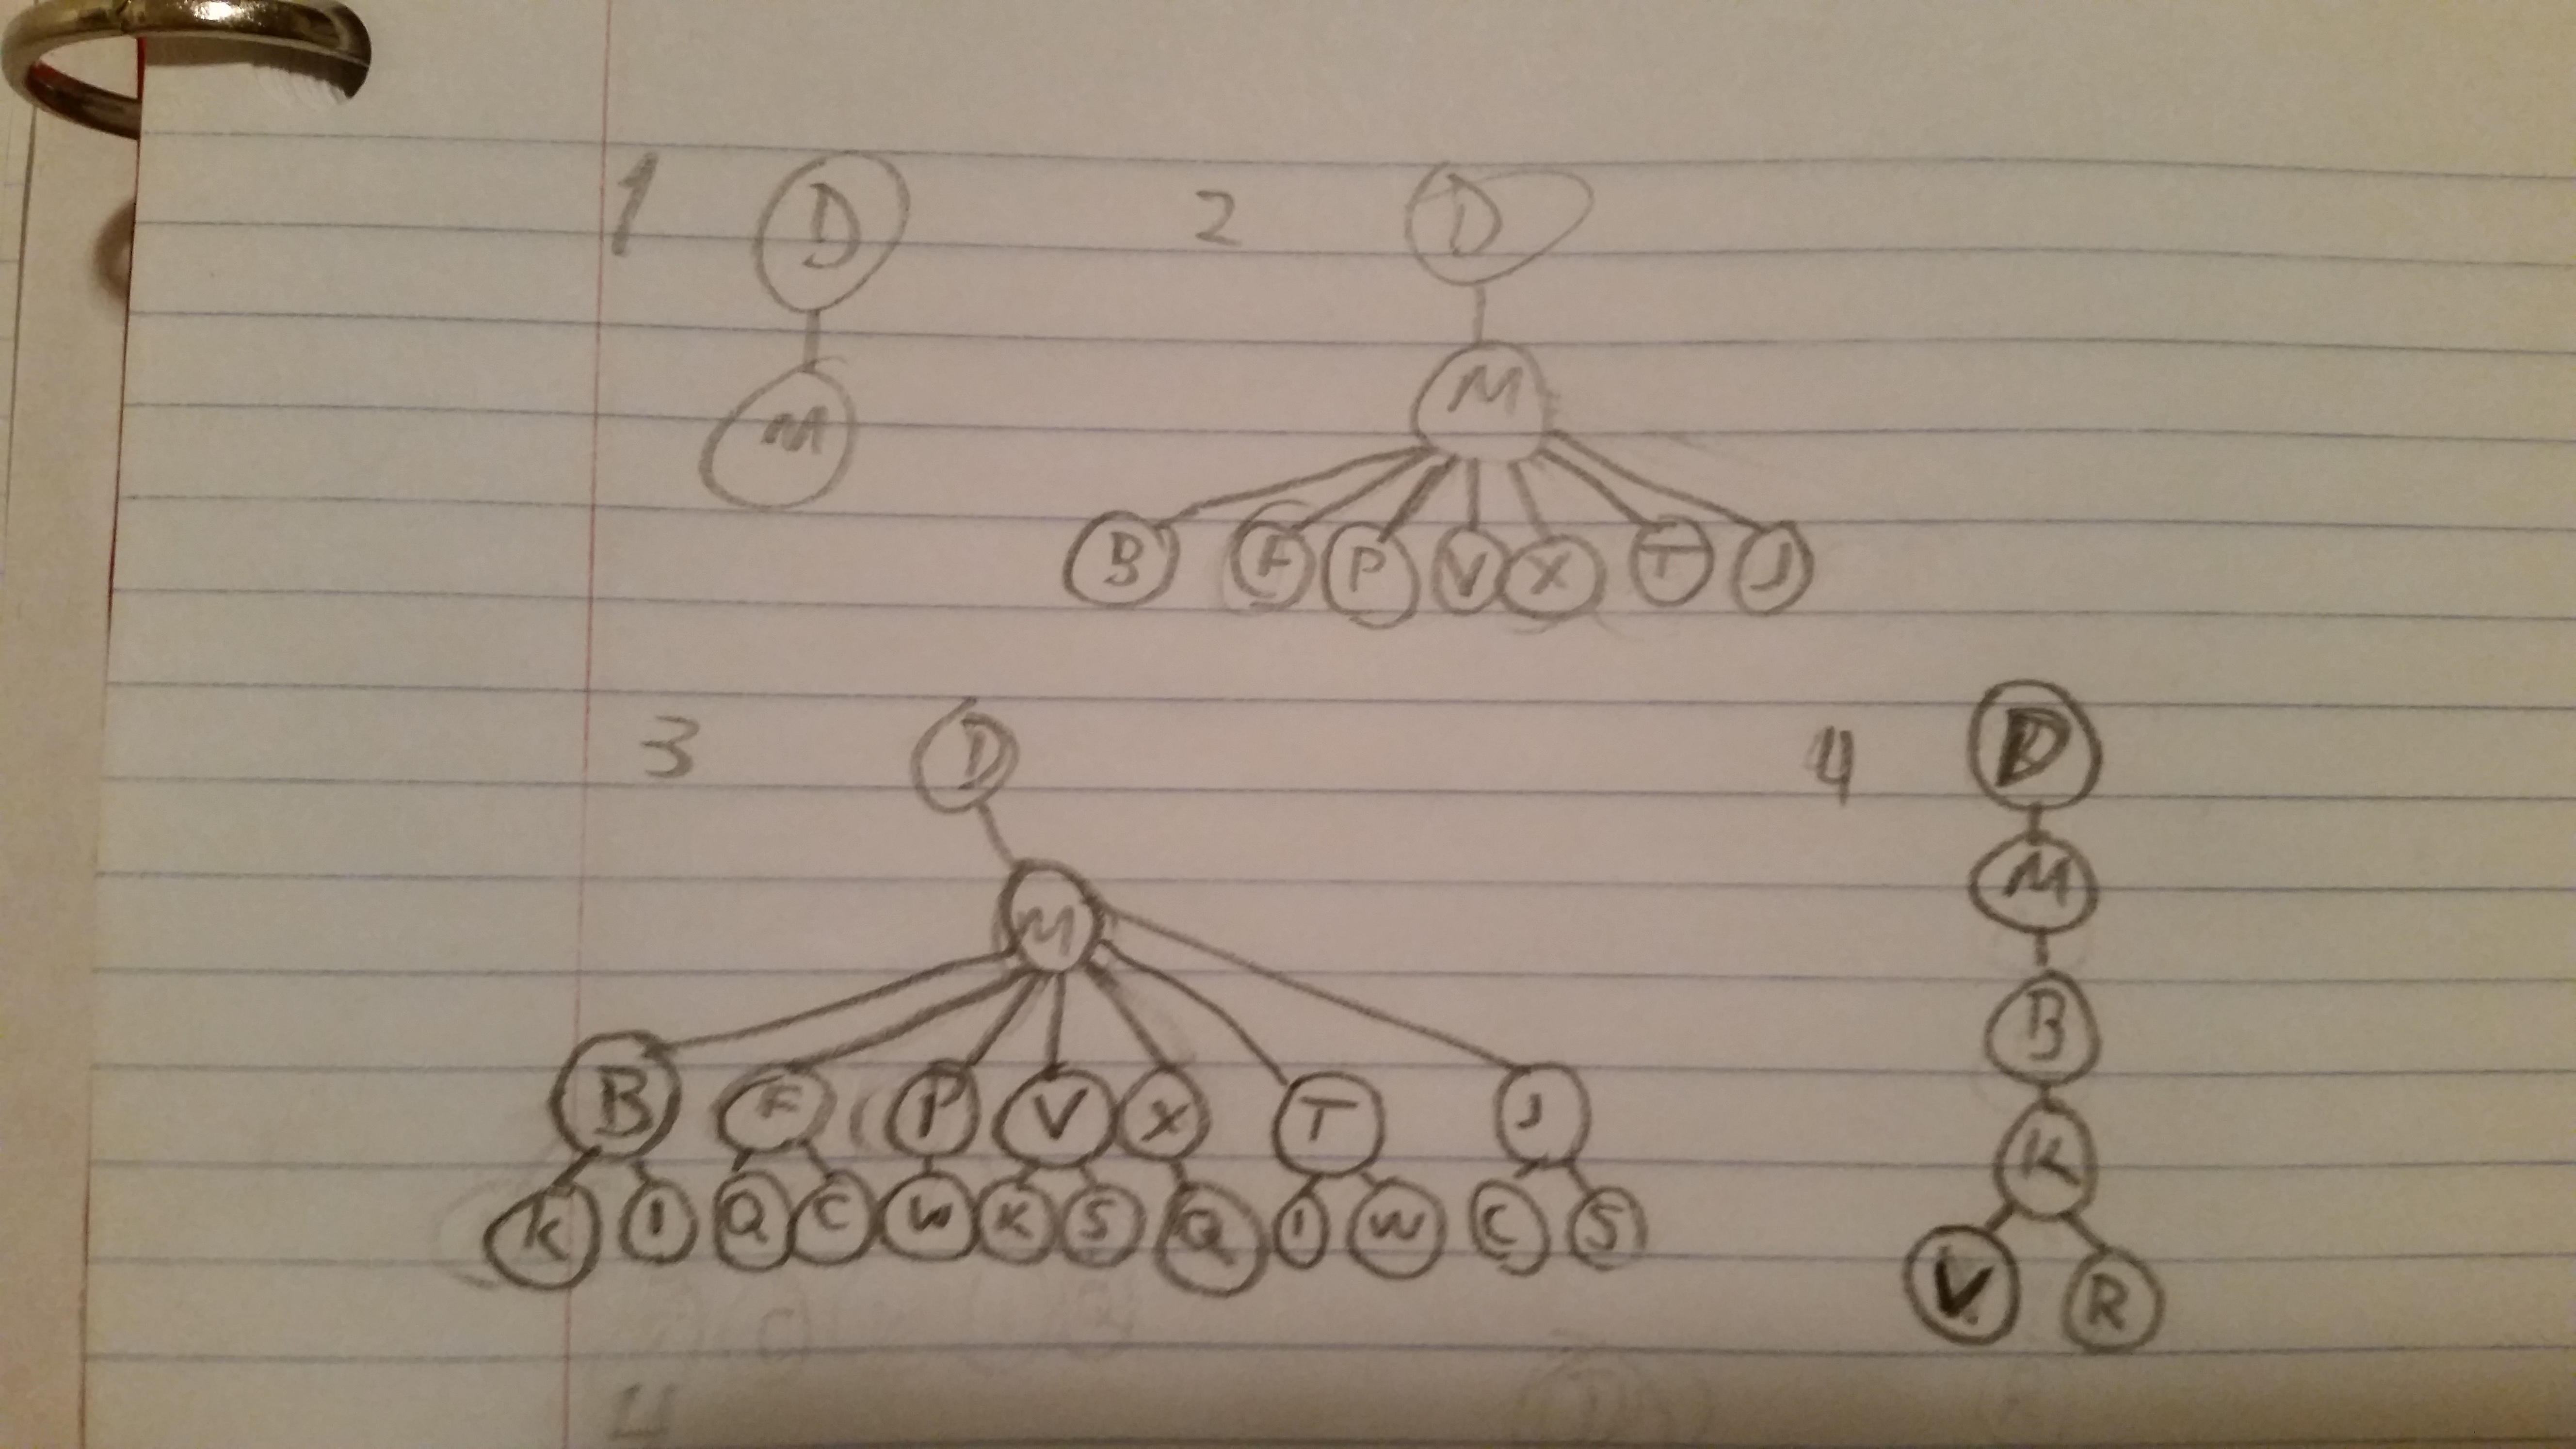
\includegraphics[width=0.9\textwidth]{1b}

        %1c
        \item No; to be admissible, an heuristic must never over-estimate the cost of a path; this heuristic will always over-estimate the cost for any square from which the knight can capture the king (the cost will be one, but the heuristic value will be three), among others.

\pagebreak

        %1d
        \item Solution path: $D{\rightarrow}M{\rightarrow}T{\rightarrow}I{\rightarrow}R$, cost 4.\\
            \begin{tabular}{|l|p{6cm}|p{7.5cm}|}
                \hline
                    Current & Frontier & Expanded \\\hline\hline
                        & D:4 ($g=0, h=4$) & \\\hline
                    D:4 & M:2 ($g=1, h=1$) & \\\hline
                    M:2 & P:4 ($g=2, h=2$), T:4 ($g=2, h=2$), V:4 ($g=2, h=2$), X:4 ($g=2, h=2$), B:6 ($g=2, h=4$), F:6 ($g=2, h=4$), J:6 ($g=2, h=4$) & D:4 \\\hline
                    P:4 & T:4, V:4, W:4 ($g=3, h=1$), X:4, B:6, F:6, J:6 & D:4, M:2 \\\hline
                    T:4 & V:4, W:4, X:4, B:6, F:6, I:6 ($g=3, h=3$), J:6 & D:4, M:2, P:4\\\hline
                    V:4 & S:4 ($g=3, h=1$), W:4, X:4, B:6, F:6, I:6, J:6, K:6 ($g=3, h=3$) & D:4, M:2, P:4, T:4\\\hline
                    S:4 & W:4, X:4, B:6, F:6, H:6 ($g=4, h=2$), I:6, J:6, K:6, L:6 ($g=4, h=2$) & D:4, M:2, P:4, T:4, V:4\\\hline
                    W:4 & X:4, B:6, F:6, H:6, I:6, J:6, K:6, L:6, N:6 ($g=4, h=2$) & D:4, M:2, P:4, T:4, V:4, S:4\\\hline
                    X:4 & Q:4 ($g=3, h=1$), B:6, F:6, H:6, I:6, J:6, K:6, L:6, N:6 & D:4, M:2, P:4, T:4, V:4, S:4, W:4\\\hline
                    Q:4 & B:6, F:6, H:6, I:6, J:6, K:6, L:6, N:6 & D:4, M:2, P:4, T:4, V:4, S:4, W:4, X:4\\\hline
                    B:6 & F:6, H:6, I:6, J:6, K:6, L:6, N:6 & D:4, M:2, P:4, T:4, V:4, S:4, W:4, X:4, Q:4\\\hline
                    F:6 & C:6 ($g=3, h=3$) H:6, I:6, J:6, K:6, L:6, N:6 & D:4, M:2, P:4, T:4, V:4, S:4, W:4, X:4, Q:4, B:6\\\hline
                    C:6 & H:6, I:6, J:6, K:6, L:6, N:6 & D:4, M:2, P:4, T:4, V:4, S:4, W:4, X:4, Q:4, B:6, F:6\\\hline
                    H:6 & I:6, J:6, K:6, L:6, N:6 & D:4, M:2, P:4, T:4, V:4, S:4, W:4, X:4, Q:4, B:6, F:6, C:6\\\hline
                    I:6 & R:4 ($g=4, h=0$), J:6, K:6, L:6, N:6 & D:4, M:2, P:4, T:4, V:4, S:4, W:4, X:4, Q:4, B:6, F:6, C:6, H:6\\\hline
                    R:4 & J:6, K:6, L:6, N:6 & D:4, M:2, P:4, T:4, V:4, S:4, W:4, X:4, Q:4, B:6, F:6, C:6, H:6, I:6\\
                \hline
            \end{tabular}
    \end{enumerate}
\end{enumerate}

\end{document}


